% 整个文档的主文件。只需要在这个地方编译一次即可。

\documentclass[openany]{ctexbook}      
% 支持中文的书籍文档类
% [openany] 就是单面打印的意思。如果把这个去掉后,
% 则每次 include 都会自动空页来保证每章第一页都在奇数页。

\usepackage{pdfpages}



\usepackage{listings}
\usepackage{xcolor} %(可选,为了高亮配色)
\lstset{
  language=C++,               % 代码类型
  basicstyle=\ttfamily\footnotesize, % 代码字体小号等宽
  keywordstyle=\color{blue},  % 关键词蓝色
  commentstyle=\color{gray},  % 注释灰色
  numbers=none,               % 行号在左
  numberstyle=\tiny\color{gray},
  breaklines=true,            % 自动换行
  frame=single,               % 框出代码区域
  columns=fullflexible,
}
% 用 listings 来展示代码

\usepackage[
    hidelinks,         % 不标色也不加框,保持外观整洁
    bookmarksopen=true,% 打开时书签默认展开
    bookmarksnumbered=true, % 书签带章节号
    unicode=true       % 书签支持Unicode,防止中文乱码
]{hyperref}

\hypersetup{
    colorlinks=true,    % 使用彩色文字(非边框)
    linkcolor=blue,     % 内部链接颜色
    urlcolor=red,       % URL链接颜色
    citecolor=magenta    % 引用颜色
}

\usepackage[top=2cm, bottom=2cm, left=2cm, right=2cm]{geometry}
% ctexbook 默认边距太大,有点浪费资源。在这里调一下

\usepackage{amsmath}
% \implies 蜜汁不能用

\title{XCPC 算法竞赛模板}
\author{Sergio Gao}



\renewcommand\contentsname{\songti\zihao{2} 目\quad 录}
\ctexset{
    chapter = {
        format = \centering\zihao{2}\songti\bfseries, % 居中,宋体,large字号
        name = {第\space, \space 章},
        number = \arabic{chapter},
    }
}
\ctexset{
    section = {
        format = \centering\zihao{-2}\songti\bfseries, 
    }
}
\ctexset{
    subsection = {
        format = \centering\zihao{-3}\songti\bfseries, 
    }
}

\begin{document}

\maketitle
\tableofcontents



\section{网络流}

网络流在 XCPC 中常考的两类:

第一类是最大流或者最小割。这类一般建完图用 Dinic 算法解决即可。

特别地,最经典的一类题型:等价于求二分图的最大匹配。
而最大匹配用最大流来跑又快又好,并且还能顺便证明二分图最大匹配 = 最小点覆盖。

二分图中:最大匹配(最大流) = 最小点覆盖(最小割) = 点数 - 最大独立集

第二类是最小费用最大流。这类一般建完图用 Dij 费用流解决即可。
大多数费用流算法都和其流 $f$ 相关。构造时一般是那最大流作为可以控制的约束。
特别地,最经典的一类题型:等价于求二分图的最大权匹配。

\section{网络流}

网络流在 XCPC 中常考的两类:

第一类是最大流或者最小割。这类一般建完图用 Dinic 算法解决即可。

特别地,最经典的一类题型:等价于求二分图的最大匹配。
而最大匹配用最大流来跑又快又好,并且还能顺便证明二分图最大匹配 = 最小点覆盖。

二分图中:最大匹配(最大流) = 最小点覆盖(最小割) = 点数 - 最大独立集

第二类是最小费用最大流。这类一般建完图用 Dij 费用流解决即可。
大多数费用流算法都和其流 $f$ 相关。构造时一般是那最大流作为可以控制的约束。
特别地,最经典的一类题型:等价于求二分图的最大权匹配。

\subsection{求强连通分量}

这是对于有向图,求出若干极大两两可互相到达的点集。

一些没有写上去但可能会用到的 trick:

对于强连通分量,存在容易算法判断是否存在非零环。
(提示:如果存在两个权值不一样的环,那么一定存在非零环。)

\lstinputlisting{Graph_Theory/tarjan/tarjan_scc.cpp}


\section{网络流}

网络流在 XCPC 中常考的两类:

第一类是最大流或者最小割。这类一般建完图用 Dinic 算法解决即可。

特别地,最经典的一类题型:等价于求二分图的最大匹配。
而最大匹配用最大流来跑又快又好,并且还能顺便证明二分图最大匹配 = 最小点覆盖。

二分图中:最大匹配(最大流) = 最小点覆盖(最小割) = 点数 - 最大独立集

第二类是最小费用最大流。这类一般建完图用 Dij 费用流解决即可。
大多数费用流算法都和其流 $f$ 相关。构造时一般是那最大流作为可以控制的约束。
特别地,最经典的一类题型:等价于求二分图的最大权匹配。

\subsection{Dinic 最大流}

一般的时间复杂度会估计到 $O(n^2 m)$,但很多题目的建图有特殊性,跑不满。
特别的,如果拿来处理二分图最大匹配,复杂度可以估到 $O(n^3)$。

\lstinputlisting{Graph_Theory/flow/dinic_flow.cpp}

\subsection{Dijkstra 费用流}

首先,费用流一般是要自己构造的,所以一般有意义的问题不会有真正的负环。
然而负权是允许的。通过调整正负,可以把最小费用流的算法改写成最大费用流。

Dijkstra 费用流也就是在保证初始能赋出一个合理的势能函数的前提下,
用 Dijkstra 来找到从源点到汇点的最短路。

最暴力的做法是初始做一遍 spfa,这个复杂度可能会达到 $O(n m)$。
或者根据题目的特殊性。
有一些问题它给出时就已经是让我们求如何最大化一些势能差之和。

除去这个初始化,复杂度是 $O(f m \log m)$。
要注意,像是二部图最大权匹配,$f$ 取决于较小的那一部,所以不要误认为其等于总点数。

\lstinputlisting{Graph_Theory/flow/dijkstra_flow.cpp}



\section{网络流}

网络流在 XCPC 中常考的两类:

第一类是最大流或者最小割。这类一般建完图用 Dinic 算法解决即可。

特别地,最经典的一类题型:等价于求二分图的最大匹配。
而最大匹配用最大流来跑又快又好,并且还能顺便证明二分图最大匹配 = 最小点覆盖。

二分图中:最大匹配(最大流) = 最小点覆盖(最小割) = 点数 - 最大独立集

第二类是最小费用最大流。这类一般建完图用 Dij 费用流解决即可。
大多数费用流算法都和其流 $f$ 相关。构造时一般是那最大流作为可以控制的约束。
特别地,最经典的一类题型:等价于求二分图的最大权匹配。

\section{网络流}

网络流在 XCPC 中常考的两类:

第一类是最大流或者最小割。这类一般建完图用 Dinic 算法解决即可。

特别地,最经典的一类题型:等价于求二分图的最大匹配。
而最大匹配用最大流来跑又快又好,并且还能顺便证明二分图最大匹配 = 最小点覆盖。

二分图中:最大匹配(最大流) = 最小点覆盖(最小割) = 点数 - 最大独立集

第二类是最小费用最大流。这类一般建完图用 Dij 费用流解决即可。
大多数费用流算法都和其流 $f$ 相关。构造时一般是那最大流作为可以控制的约束。
特别地,最经典的一类题型:等价于求二分图的最大权匹配。

\subsection{四边形不等式优化 DP}

\href{https://loj.ac/p/2157}{2157. 「POI2011 R1」避雷针 Lightning Conductor - 题目 - LibreOJ}

这个情景是,下标决策点未必是要小于当前点的。
这种问题只需要正向跑一边,逆向跑一边,在两者之间取更优即可。
模板是解决前面标准的
\begin{itemize}
    \item 四边形不等式指 相交 $\le$ 包含
    \item 等价于要决策的是最小值
\end{itemize}

注意中途运算时 sqrt 相关操作不能取整,反之则会破坏 $-\sqrt{x}$ 的下凸性(比如说相邻两项点值一样斜率就直接为 0 了)。

\lstinputlisting{Convex_Optimization/monge/monge_dp.cpp}
\subsection{预备节:WQS 二分}

\href{https://www.luogu.com.cn/problem/P2619}{P2619 [国家集训队]Tree I - 洛谷}

洛谷题解质量有点差,很多都看不出和 wqs 二分有什么关系。

这样思考,设 $g_x$ 是恰选中 $x$ 条白边的最小权。那么 $f(x) := g_x - \lambda x$ 就是给这 $x$ 条白边的权值减去 $\lambda$ 的惩罚代价后的权值,那么 $g_x-\lambda x$ 的最小值在什么地方取到?这等价于提前给所有白边都减去 $\lambda$,然后跑 mst。这有什么意义呢?

考虑 $(need-1, g_{need-1})$ 和 $(need, g_{need})$,当 $\lambda$ 恰好等于这两个点的斜率时,如果能有下凸性,并且同取最小值的时候可以取 $x$ 大的,这时候就会取到后面的那个作为最小值的 $x$ 点(如果取到 $>need$ 的其实同理可以往回取)。

当 $\lambda$ 大于这两个点的斜率时,$< need$ 的部分 比 大于等于 $\ge need$ 的部分不优。

当 $\lambda$ 大于这两个点的斜率时,$< need$ 的部分 比 大于等于 $\ge need$ 的部分更优。

所以二分这个惩罚代价,使得 $p = \max\{pos : f(pos) = \min_{x}\{f(x)\}\}$ 位于 $\ge need$ 部分,那么必然通过调整使得 $f(need) = f(p)$。

貌似有道更难一点的:\href{https://www.luogu.com.cn/problem/P5633}{P5633 最小度限制生成树 - 洛谷}。

\href{https://www.luogu.com.cn/problem/P1912}{P1912 [NOI2009] 诗人小G - 洛谷}

\href{https://www.luogu.com.cn/article/e362a4cs}{题解 P1912 【[NOI2009]诗人小G】 - 洛谷专栏}

\lstinputlisting{Convex_Optimization/monge/wqs_binary_search.cpp}
\subsection{WQS 二分结合决策单调性}

这个属于是固定套路,区间分划问题。下面给出对应模板代码情景的题解。

\href{https://codeforces.com/gym/105486/problem/F}{2024 Chengdu Regional F} 

考虑到

$$
(\sum\limits_{i=1}^{m}\frac{num_i}{k_i}) (\sum\limits_{i=1}^{m}k_i sum_i) \ge (\sum_{i=1}^{m}\sqrt{num_i\cdot sum_i})^2
$$
因为要最小化 $\sum\limits_{i=1}^{m}\frac{num_i}{k_i}$ 所以用调整法可以说明 $(\sum\limits_{i=1}^{m}k_i sum_i)$ 会取其上界 $1$,这就把 $\{k\}$ 给安排了。
只需要最小化右式子。再用调整法可以说明 sum 里面应该是连续的,于是可以先对 $s$ 排序,然后按顺序做一个 dp。这实际上就转化成了一个限制区间个数的区间分拆问题

WQS 二分,引入一个惩罚参数 lambda,将问题转化为:不限制分组数,但每多一组就要付出 lambda 的代价。可以看出惩罚参数越大分组越少,所以我们大概是要求一个适当大的惩罚参数使得分组的组数不超过 $m$。

这里的四边形不等式貌似不能直接套结论把 $\sqrt{x}$ 剥掉直接考虑 $x$,因为这里就是要考虑 $w(i,j) = dp[i-1] + \sqrt{(j-i)(pre_{j} - pre_{i})} + \lambda$ 这样的 $w$ 取 min,而不带负号 sqrt 并非下凸而是上凸。
当然这里还是只需要考虑 $\sqrt{(j-i)(pre_{j} - pre_{i})}$ 是否满足四边形不等式。
直观地理解的话,把 $pre_j$ 替换成 $j$,于是 $w$ 刚好到 $j-i$,一个凸性的临界点。然后 $pre$ 可能会再稍微下凸一点,即考虑到 $\Delta pre$ 单调不减,就让这个 $w$ 变成下凸的了。

然后就是一个典型的区间分拆问题,这类问题\textbf{听说}只要把四边形不等式证出来了,则可推出 Monge 最短路关于 经过的边数 $k$(即拆分组数)有下凸性。
这题貌似没有说清楚能不能让 $num_i=0$,即某个区间为空,即只需要区间数 $\le m$ 而非恰好 $m$。但看起来通过一点调整可以说明组数越多越好。所以关于组数应该是一个下凸的减函数。

\lstinputlisting{Convex_Optimization/monge/wqs_monge_dp.cpp}
\section{网络流}

网络流在 XCPC 中常考的两类:

第一类是最大流或者最小割。这类一般建完图用 Dinic 算法解决即可。

特别地,最经典的一类题型:等价于求二分图的最大匹配。
而最大匹配用最大流来跑又快又好,并且还能顺便证明二分图最大匹配 = 最小点覆盖。

二分图中:最大匹配(最大流) = 最小点覆盖(最小割) = 点数 - 最大独立集

第二类是最小费用最大流。这类一般建完图用 Dij 费用流解决即可。
大多数费用流算法都和其流 $f$ 相关。构造时一般是那最大流作为可以控制的约束。
特别地,最经典的一类题型:等价于求二分图的最大权匹配。

\subsection{李超线段树}

\subsubsection{值域 $10^6$,针对线段}

要求在平面直角坐标系下维护两个操作:

\begin{itemize}
    \item 在平面上加入一条线段。记第 $i$ 条被插入的线段的标号为 $i$。
    \item 给定一个数 $k$,询问与直线 $x = k$ 相交的线段中,交点纵坐标最大的线段的编号。
\end{itemize}

\lstinputlisting{Convex_Optimization/Convex_Datastructure/lichao_tree1.cpp}

这个模板其实可能不够好,也不常用。主要是它的时间复杂度会和定义域大小相关。有些问题要查 1e9 就寄了。

\subsubsection{值域 $10^9$,针对直线}

更常用的应该是没有定义域限制,功能一样,然后拿来优化一些 dp。

下面这个模板展示了原来的 dp 和用李超线段树优化后的用法。

\href{https://codeforces.com/contest/2107/problem/F2}{CF2107F2}

\lstinputlisting{Convex_Optimization/Convex_Datastructure/lichao_tree2.cpp}

有的人会误认为内存要开成 $N\log V$,其中 $V$ 为 $10^9$,而大多数情况下存一个直线是需要至少一个 int 一个 long long 的,如果 $N$ 是 $10^6$ 再乘个 30 就很容易炸。实际上这是一种误解。

仔细观察实现过程,这个线段树没有分割后分别递归,而是只会往一侧走。

每次存下直线后都会直接停止,从而可以知道每次 add 操作只会新建一个结点,所以内存开成 $N$ 即可。

另外还有一个经典问题

Q:这种问题可能是什么原因,孩子调半天没搞明白

\begin{itemize}
    
\item 想用 vector 动态开点,每次用 .size() 来得到当前的 id(本地测试能出正确答案,OJ 上 RE)

\item 也是 vector,但是定义的时候预先定义大小,另外开一个 int 类型来记录当前 id(本地测出来和 1 一样,OJ 上 AC)

\end{itemize}

A:递归中存在对 vector 的引用,结果中途给 vector 扩容了,导致引用失效。


\section{网络流}

网络流在 XCPC 中常考的两类:

第一类是最大流或者最小割。这类一般建完图用 Dinic 算法解决即可。

特别地,最经典的一类题型:等价于求二分图的最大匹配。
而最大匹配用最大流来跑又快又好,并且还能顺便证明二分图最大匹配 = 最小点覆盖。

二分图中:最大匹配(最大流) = 最小点覆盖(最小割) = 点数 - 最大独立集

第二类是最小费用最大流。这类一般建完图用 Dij 费用流解决即可。
大多数费用流算法都和其流 $f$ 相关。构造时一般是那最大流作为可以控制的约束。
特别地,最经典的一类题型:等价于求二分图的最大权匹配。

\section{网络流}

网络流在 XCPC 中常考的两类:

第一类是最大流或者最小割。这类一般建完图用 Dinic 算法解决即可。

特别地,最经典的一类题型:等价于求二分图的最大匹配。
而最大匹配用最大流来跑又快又好,并且还能顺便证明二分图最大匹配 = 最小点覆盖。

二分图中:最大匹配(最大流) = 最小点覆盖(最小割) = 点数 - 最大独立集

第二类是最小费用最大流。这类一般建完图用 Dij 费用流解决即可。
大多数费用流算法都和其流 $f$ 相关。构造时一般是那最大流作为可以控制的约束。
特别地,最经典的一类题型:等价于求二分图的最大权匹配。

\subsection{最小公共圆}

一个期望复杂度正确的随机化算法

\lstinputlisting{Computing_Geometry/random_methods/least_common_circle.cpp}

\section{网络流}

网络流在 XCPC 中常考的两类:

第一类是最大流或者最小割。这类一般建完图用 Dinic 算法解决即可。

特别地,最经典的一类题型:等价于求二分图的最大匹配。
而最大匹配用最大流来跑又快又好,并且还能顺便证明二分图最大匹配 = 最小点覆盖。

二分图中:最大匹配(最大流) = 最小点覆盖(最小割) = 点数 - 最大独立集

第二类是最小费用最大流。这类一般建完图用 Dij 费用流解决即可。
大多数费用流算法都和其流 $f$ 相关。构造时一般是那最大流作为可以控制的约束。
特别地,最经典的一类题型:等价于求二分图的最大权匹配。

\section{网络流}

网络流在 XCPC 中常考的两类:

第一类是最大流或者最小割。这类一般建完图用 Dinic 算法解决即可。

特别地,最经典的一类题型:等价于求二分图的最大匹配。
而最大匹配用最大流来跑又快又好,并且还能顺便证明二分图最大匹配 = 最小点覆盖。

二分图中:最大匹配(最大流) = 最小点覆盖(最小割) = 点数 - 最大独立集

第二类是最小费用最大流。这类一般建完图用 Dij 费用流解决即可。
大多数费用流算法都和其流 $f$ 相关。构造时一般是那最大流作为可以控制的约束。
特别地,最经典的一类题型:等价于求二分图的最大权匹配。

\subsection{找模素数 P 的原根}

首先必然素数 $P$ 必然有原根。
据说可以证明最小的原根的数量级大概是 $O(P^{1/4})$,
然后考虑到 Fermat 小定理给出的 $p-1$ 必然是阶的倍数,
所以可以暴力枚举其因数判断阶是否小于 $p-1$。

\lstinputlisting{Math/number_theory/primitive_root.cpp}
\subsection{杜教筛求 premu}


\lstinputlisting{Math/algorithms/number_theory/dujiao_sieve.cpp}

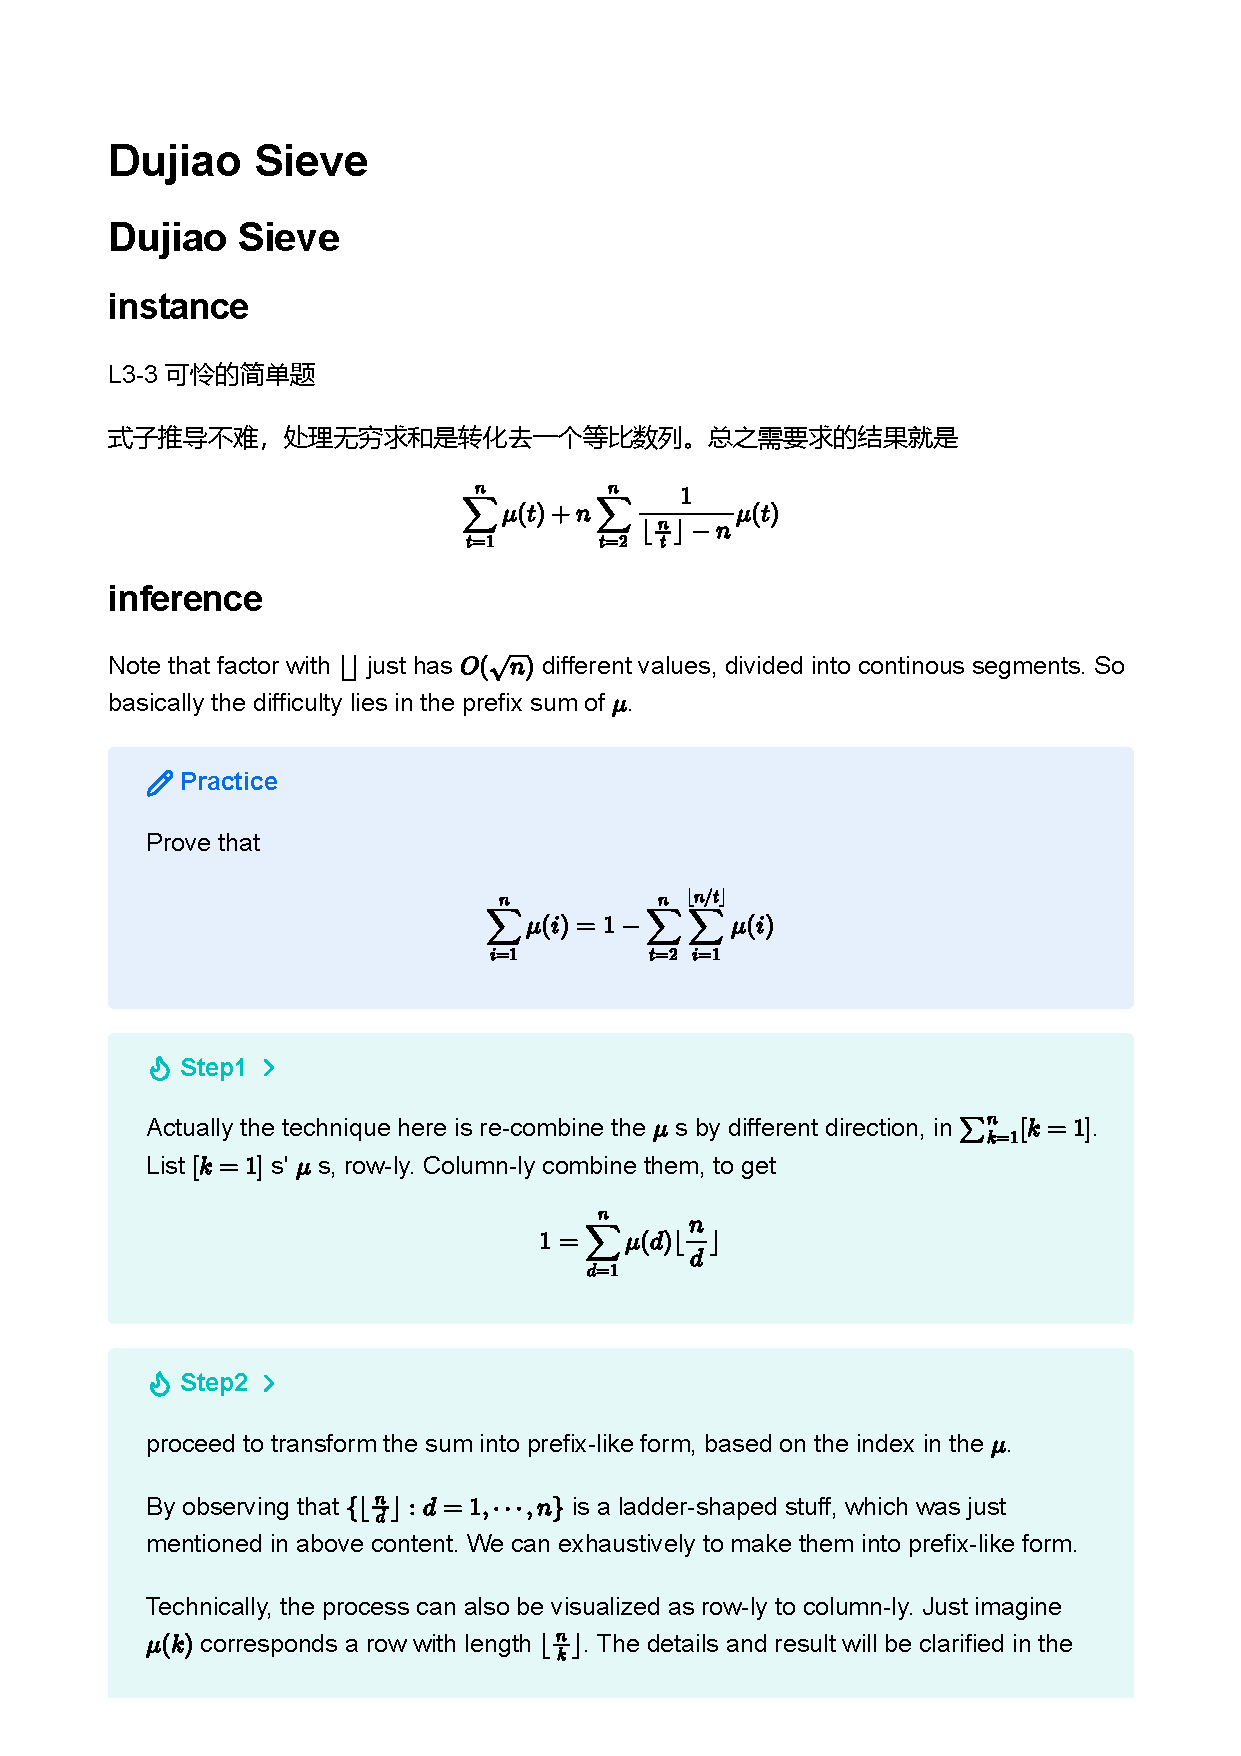
\includepdf[pages=-]{Math/algorithms/number_theory/dujiao_sieve.pdf}
\section{网络流}

网络流在 XCPC 中常考的两类:

第一类是最大流或者最小割。这类一般建完图用 Dinic 算法解决即可。

特别地,最经典的一类题型:等价于求二分图的最大匹配。
而最大匹配用最大流来跑又快又好,并且还能顺便证明二分图最大匹配 = 最小点覆盖。

二分图中:最大匹配(最大流) = 最小点覆盖(最小割) = 点数 - 最大独立集

第二类是最小费用最大流。这类一般建完图用 Dij 费用流解决即可。
大多数费用流算法都和其流 $f$ 相关。构造时一般是那最大流作为可以控制的约束。
特别地,最经典的一类题型:等价于求二分图的最大权匹配。

\subsection{NTT}

主要的部分就是算一个特殊的矩阵乘向量得到的向量
void ntt(vector a, bool invert 因为逆矩阵几乎一样,方法通用,就写进一个函数里 )
记录一下 a 的大小 n。实际上这里的 n 会在后面调用的时候提前变成 2 的幂次。

先作一个预处理,所谓蝴蝶操作。就是后面我们会把系数根据奇偶位分成两份多项式,直到拆到底层成为一个直接可以引用的下标。我们把这个下标提前放好,后面就可以迭代地自下往上了。
这里先直观给出小例子

0 → 000 → 000 → 0  

1 → 001 → 100 → 4  

2 → 010 → 010 → 2  

3 → 011 → 110 → 6  

4 → 100 → 001 → 1  

5 → 101 → 101 → 5  

6 → 110 → 011 → 3  

7 → 111 → 111 → 7

大致上是一个两两配对并 swap 的过程。我们可以只枚举小的然后去找对应大的,防止 swap 两次结果还原了。只要能做到 $O(n\log n)$ 就行了,这里的实现方法可以是:考虑我给 $i$ 从 $0$ 开始加实际上在干什么:从右往左找到第一个 0,变成 1,然后抹掉这个位置以右的位置。镜面地对另一个 $j$ 从 $0$ 开始操作,就能得到镜面的结果了。

从最短 len=2 开始往 n 合并,每次 len 倍长。
假设已经计算出了 $len/2$ 的奇数项多项式和偶数项多项式。现在来计算 len 的多项式。
记当前单位根是 $w_{len}$,实质上对于 $f(w_{len}^{k})$,我们需要的是 $f(w_{len}^{k}) = f_1(w_{len/2}^{k}) +w_{len}^{k}f_2(w_{len/2}^{k})$。对于 $k<len/2$ 我们就直接引用对应位置的点值来计算;对于 $k\ge len/2$ 的,考虑到 $w_{len/2}^{k} = w_{len/2}^{k-len/2}$,$w_{len}^{k} = -w_{len}^{k-len/2}$,可以引用对应点值,也可以在在处理 $k-len/2$ 时顺便处理了,并且这样的话就可以直接覆盖掉对应的位置而不怕后面还会被引用了。

模意义下的单位根 $w_{len}$ 是什么意思呢?NTT 模数 $p$ 减一,即 998244353-1 后是 $2^{23}\approx 8e6$ 的倍数,大于算法竞赛环境下 $O(n\log n)$ 复杂度允许的 $n$;
$3$ 又是这个模数的原根,即第一个循环节刚好是费马小定理指出的一个循环节 $p-1$,
所以我们可以指定 $w_{len} = 3^{(p-1)/len}$,并验证它符合我们需要的各种单位根性质。稍微强调一下:最主要的动机在于
$$
\sum_{k=0}^{n-1}(w_n^{i-j})^{k}
$$
应该需要在 $i=j$ 时为一个统一的常数,而在 $i\not=j$ 时为 $0$,即这时
$$
w_{n}^{i-j}\not= 1 \land w_{n}^{(i-j)n}=1
$$
加入让 $w_{len}=g^{(p-1)/len}$,其中 $g$ 不是原根的话,$g^{(i-j)(p-1)/n}$,这里 $(i-j)$ 的取值范围实际上是 $-(n-1)$ 到 $(n-1)$,就有可能撞上一个比 $p-1$ 小的循环节,让这个结果变成 $1$ 了。
这个动机实质上就是在验证这个形式的矩阵是否真的是逆矩阵。对于原根打底的,那确实是。反之,要么我们通过上面的解剖来验证伪,要么就直接考虑一下矩阵中存在完全相同的某两行,那么行列式为 $0$,必然不存在逆矩阵。


如果是 invert 的话实质上求逆时还会多一项公因数 $1/n$(其实就是我们先前提到的统一常数),所以每项结果再乘一下就好了。

下面顺便把半在线卷积以及可以利用半在线卷积实现的功能写上去了。实际上现场推也并不困难。

\lstinputlisting{Math/polynomials/NTT.cpp}

% 我的文件管理规范:
% 对于大类,新建一个文件夹。
% 里面写一个 intro.tex,新起一个 chapter,顺便来介绍这个大类的总体内容
% 然后再建一个二级文件夹。
% 里面放各种算法的 .tex 和 .cpp
% 同理可以再在建三级文件夹。一般不建议四级以上


\end{document}


